\section{CONCEPTOS GENERALES}

\subsection{Machine Learning}
Conocemos como Machine Learning a la rama de la computación que estudia el diseño de algoritmos que son capaces de aprender. Este tipo de algoritmos son utilizados en la actualidad para muchas aplicaciones, por ejemplo para recomendaciones de películas o para ranquear sitios web en base a una consulta.


\subsection{Algoritmo y Modelo}

Se parte de un algoritmo de Machine Learning y se desea obtener lo que conocemos como modelo, aquel que se adapte mejor a nuestro set de datos. El algoritmo es el enfoque general que se toma. El modelo es lo que se obtiene cuando se ejecuta el algoritmo sobre el set datos de entrenamiento y lo que se usa para hacer predicciones sobre nuevos datos. Se puede generar un nuevo modelo con el mismo algoritmo pero con datos diferentes, o un modelo diferente de los mismos datos con un algoritmo diferente. 
Cada modelo tiene un conjunto de parámetros e hiper-parámetros que necesita para funcionar. Los parámetros los descubre el algoritmo a partir de los datos, los hiper-parámetros, en cambio, son datos que debemos pasarle al algoritmo para funcionar\footnote{Apunte del curso, 11.1
Evaluación de Algoritmos de ML}. Por lo tanto la clave está en encontrar los hiper-parámetros óptimos.


\subsection{Árboles de Decisión}

Los árboles de decisión son un tipo algoritmos de aprendizaje supervisado donde en cada nodo se va dividiendo el conjunto de datos en dos o más sub-conjuntos siguiendo un criterio de particionamiento, se procede asi para cada sub-conjunto derivado, creando nodos hasta cumplir ciertas condiciones de corte donde se definen las hojas del árbol. Son mayormente usados para problemas de clasificación pero también dan excelentes resultados para casos de regresión.

Estos árboles, una vez preparados con un set de entrenamiento, están listos para realizar categorizaciones o predicciones de variables continuas según el caso. Son sensibles a los datos con los que fue entrenado, es decir, ante cambios en estos últimos los resultados del árbol pueden variar.

Existen muchas formas de realizar las divisiones en los nodos. Lo importante es generar las particiones a partir de la característica que mejor resultados nos pueda brindar. Para encontrar cuál es la óptima se recurren a técnicas matemáticas como el cálculo del desvío para cada clase. Se entiende que para cada nodo i de un árbol de decisión las k clases del sub-conjunto de datos tienen una distribución de probabilidades a la cuál es posible calcularle su desviación, entonces podríamos decir que la que resulte mayor es la mejor opción para dividir. 

\begin{figure}[h!]
\centering
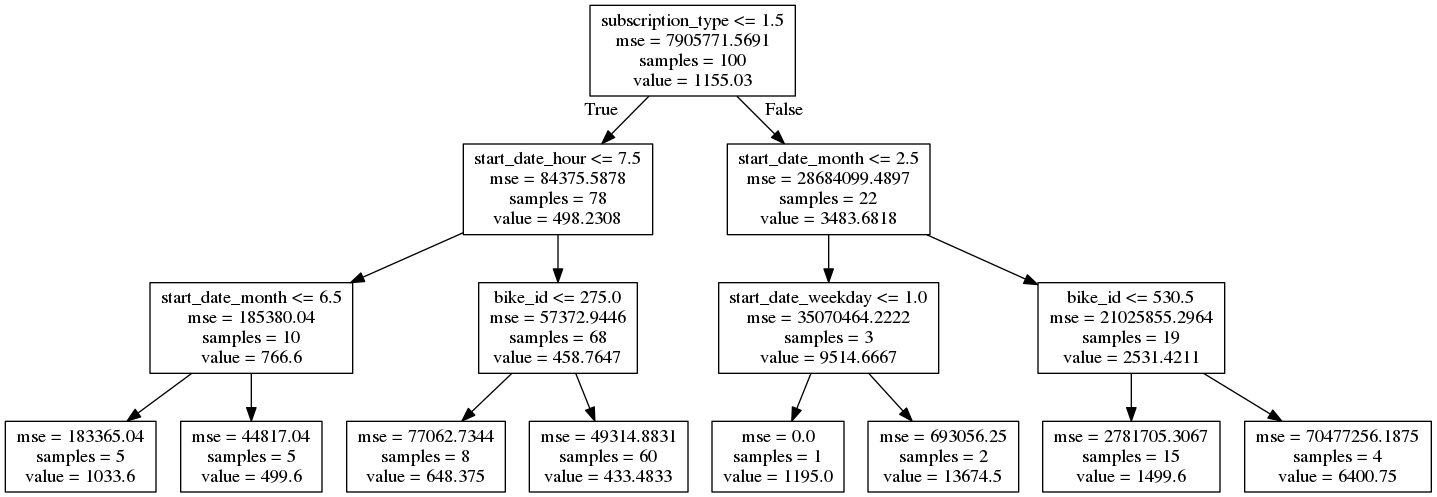
\includegraphics[width=165mm]{imagenes/tree.png}
\end{figure}


\subsection{Bootstrap Method}

Explicación del método usado para los splits
The bootstrap is a powerful statistical method for estimating a quantity from a data sample. This is easiest to understand if the quantity is a descriptive statistic such as a mean or a standard deviation.

\subsection{Método de Ensamblado}
An ensemble method is a technique that combines the predictions from multiple machine learning algorithms together to make more accurate predictions than any individual model.


\subsubsection{Bagging}

https://rafalab.github.io/pages/649/section-11.pdf

steps:
Create many (e.g. 100) random sub-samples of our dataset with replacement.
Train a CART model on each sample.
Given a new dataset, calculate the average prediction from each model.

when selecting a split point, the learning algorithm is allowed to look through all variables and all variable values in order to select the most optimal split-point

https://pdfs.semanticscholar.org/47a1/979c3f7778232c2f038530ff1bb67f235ffa.pdf

http://isoft.postech.ac.kr/Course/CS704/related_papers/BAGGING_PREDICTORS.pdf

https://github.com/rasbt/python-machine-learning-book/blob/master/faq/bagging-boosting-rf.md

https://onlinecourses.science.psu.edu/stat857/node/180


\subsubsection{Random Forest}

The number of features that can be searched at each split point (m) must be specified as a parameter to the algorithm. You can try different values and tune it using cross validation.

For classification a good default is: m = sqrt(p)
For regression a good default is: m = p/3
Where m is the number of randomly selected features that can be searched at a split point and p is the number of input variables. For example, if a dataset had 25 input variables for a classification problem, then:

m = sqrt(25)
m = 5


\subsection{Cross Validation}

El proceso de K-fold Cross Validation comienza particionando el set de entrenamiento en k bloques, luego vamos a realizar varias iteraciones en las cuales entrenamos nuestro algoritmo con k 1 bloques y lo validamos con el restante \footnote{Apunte del curso,11.1.1
Cross Validation}.

\begin{figure}[h]
\centering
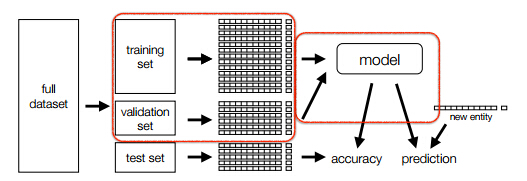
\includegraphics[height=4.5cm]{imagenes/crossValidation}
\caption{Cross Validation esquema}
\label{fig:exemplo}
\end{figure}

Este método será utilizado a en el desarrollo de este trabajo práctico. Más adelante explicaremos el porqué usarlo y los beneficios que trae.

